\documentclass[12pt]{article}
\usepackage{indentfirst}
\usepackage{fullpage}
\usepackage{multicol,multirow}
\usepackage{tabularx}
\usepackage{ulem}
\usepackage[utf8]{inputenc}
\usepackage[russian]{babel}
\usepackage{listings}
\usepackage{color}
\usepackage{graphicx}
\DeclareGraphicsExtensions{.png,.jpg}

\begin{document}
\begin{titlepage}
	\begin{center}
		\bfseries
		
		{\Large Московский авиационный институт\\ (национальный исследовательский университет)
			
		}
		
		\vspace{48pt}
		
		{\large Факультет информационных технологий и прикладной математики
		}
		
		\vspace{36pt}
		
		
		{\large Кафедра вычислительной математики и~программирования
			
		}
		
		
		\vspace{48pt}
		
		Курсовая работа по курсу <<Дискрeтный анализ>>: Методы сжатия данных
	\end{center}
	
	\vspace{72pt}
	
	\begin{flushright}
		\begin{tabular}{rl}
			Студент: & О.\,Р. Лисовский  \\
			Преподаватель: & Н.\,А. Зацепин \\
			Группа: & М8О-408Б \\
			Дата: & \\
			Оценка: & \\
			Подпись: & \\
		\end{tabular}
	\end{flushright}
	
	\vfill
	
	\begin{center}
		\bfseries
		Москва, \the\year
	\end{center}
\end{titlepage}

\pagebreak

\subsection*{Условие}

Необходимо реализовать два известных метода сжатия данных для сжатия одного файла. 

Формат запуска должен быть аналогичен формату запуска программы gzip, должны быть поддержаны следующие ключи: -c, -d, -k, -l, -r, -t -1 -9. Должно поддерживаться указание символа дефиса в качестве стандартного ввода.

\subsection*{Метод решения}

Как и требуется в условии запуск программы аналогичен запуску утилиты gzip: ./main <ключи> <файлы> <ключи> <файлы> ...

\subsubsection*{Обработка входных данных}

Первоначально программа обрабатывает то, что получает на входе, отделяя имена файлов и директорий от введённых ключей. Ключи от файлов программа отделяет по первому символу слова: если этот символ является <<->>, то полученное слово является набором ключей. В процессе изучения поведения утилиты gzip я вывел следующее дерево приоритетов ключей:

\begin{figure}[h!]
	\centering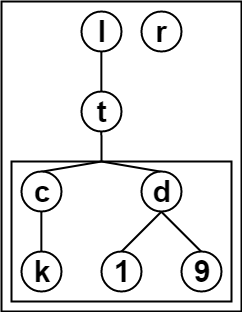
\includegraphics[scale=0.5]{KeyTree}
\end{figure}

%TODO у кого-то будет эксель табличка чтоб не так сильно палиться
Т. е. если уже был введён ключ -t, то далее ключи -c, -k, -d, -1, -9 программа учитывать не будет, но если вы ввели ключ -l, то он делает ключи -c, -k, -d, -t, -1, -9 недействительными как сейчас, так и при их будущих вводах. В то же время сочетания -cd, -c1, -c9, -kd, -k1, -k9, а так же сочетания ключа -r со всеми остальными ключами не являются взаимоисключающими. Если же во время обработки ключей встречается неизвестный ключ, то программа прекращает свою работу с соответствующей ошибкой, как и утилита gzip.

Если же полученное слово не начинается с символа <<->>, то программа идентифицирует его как имя файла/директории и заносит в красно-чёрное дерево для последующей обработки.

Для того, чтобы программа обработала файл, имя которого начинается с <<->>, необходимо ввести <<./ИМЯ\_ФАЙЛА>>.

\subsubsection*{Общий препроцессинг}

После обработки всех полученных слов программа проверяет красно-чёрное дерево на пустоту: если оно пустое, то программа завершается с соответствующим сообщением. Если же оно не пустое, то программа начинает обрабатывать все строки в данном дереве по следующему алгоритму: проверяется принадлежит ли имя директории - если нет, то это имя файла, и в дальнейшем оно обрабатывается как файл; если же это имя принадлежит директории, то проверяется активность ключа -r: если он активен, то с данной директорией идёт работа, иначе она игнорируется, и выводится соответствующее сообщение.

Работа с директорией сводится к получению всех имен файлов и директорий из неё, кроме имён <<.>> <<..>> - они пропускаются. Работа с директориями повторяет вышеописанную.

Работа с файлами во многом зависит от введённых ключей. 

\subsubsection*{Препроцессинг компрессии}

Если введённые ключи говорят о необходимости компрессии, то при отсутствии ключа -c производится проверка на наличие у файла суффикса <<.gz>>. Если он присутствует, то файл не обрабатывается, и выводится соответствующее сообщение. Если же у этого файла нет расширения <<.gz>>, то при отсутствии ключа -c проверяется наличие файла, имя которого отличается от полученного только стоящим в конце суффиксом. Если такой файл не найден, то работа продолжается. Если же он найден, то пользователю предлагается сделать выбор - перезаписывать данный файл или нет. В случае отрицательного ответа работа с данным файлом прекращается. Далее, при отсутствии ключей -1 и -9 поочерёдно происходит компрессия файла с помощью обоих алгоритмов компрессии (они будут описаны ниже вместе с алгоритмами декомпрессии). В случае провала любого алгоритма компрессии работа с файлом прекращается, и выводится соответствующая ошибка. Если же оба алгоритма сработали нормально, то при отсутствии ключа -c выбирается временный файл, созданный алгоритмами, с меньшим размером, и именно он получает расширение <<.gz>>, а файл с большим размером удаляется. Так же проверяется наличие ключа -k. При его отсутствии изначальный файл удаляется. При наличии ключей -1 или -9 отличия заключаются в том, что применяется только один из алгоритмов: -1 -- LZ77, -9 -- арифметическое кодирование.

\subsubsection*{Препроцессинг декомпрессии}

Если же ключи указывают на необходимость декомпрессии, то в случае отсутствия ключа -c и наличии ключа -d проверяется наличие у файла суффикса <<.gz>>. При выполнении всех этих условий работа с файлом прекращается, и выводится соответствующее сообщение. Далее при отсутствии ключей -t и -c проверяется наличие файла с таким же именем, но без расширения <<.gz>>. Если такой файл есть, то пользователю предлагается сделать выбор о его перезаписи. В случае отказа, работа с данным файлом прекращается, и выводится соответствующее сообщение. Если ответ положительный или такого файла нет, то работа продолжается. Из поступившего архива считывается первый байт, который содержит указание на метод архивации. Если этот байт интерпретируется как символ <<L>> или <<A>>, то декомпрессия производится по алгоритму LZ77 или Арифметика соответственно. Если первый байт интерпретируется иначе, то работа с файлом прекращается, и выводится соответствующее сообщение. В случае неудачного завершения алгоритма, выводится соответствующее сообщение и при отсутствии ключей -t и -c удаляется файл, в который записывались данные после декомпрессии, и работа с файлом прекращается. Далее при отсутствии ключей -t, -c и -k, удаляется изначальный архив, а при отсутствии ключей -t и -c временный файл для декомпрессии переименовывается и получает имя изначального архива без расширения <<.gz>>.

\subsubsection*{Получение информации об архиве}

В случае указания ключа -l производятся следующие действия. Читается первый байт, и в случае, если он не совпадает с буквами, указывающими на метод архивации, то работа прекращается, и выводится соответствующее сообщение. Далее читается 8 байт, в которые помещается размер файла до компрессии. После программа считывает размер архива, и вычисляется процент сжатия. Далее выводятся размер сжатого файла, размер до компрессии, процент сжатия в полуинтервале $[-100\%; 100\%)$ и имя файла до архивации (если файл имеет расширение <<.gz>>, то имя выводится без этого расширения, в противном случае выводится имя архива).

Далее незакодированный файл будет упоминаться как файл, а закодированный файл как архив.%TODO возьмите на вооружение

\subsubsection*{LZ77 компрессия}

\subsubsection*{LZ77 декомпрессия}

По окончании чтения архива, количество байт, которое было в изначальном файле, сверяется с тем, сколько было записано в его новую версию. При несовпадении выводится соответствующее сообщение, и декомпрессия завершается неудачно.

%TODO куда записать принцип рабты с файлами? и напишите ниже про свои алгоритмы

\subsection*{Описание файлов программы}

Код программы разбит на 11 %TODO перетасовать и объединить
 файлов:

\begin{enumerate}
	\item Arithmetic.h - Содержит перечисление методов и описание класса TArithmetic, необходимого для работы арифметической компрессии и декомпрессии. 
	\item Arithmetic.cpp - Содержит реализацию всех методов класса TArithmetic.
	\item BFile.h - Содержит перечисление методов и описание класса TOutBinary и класса TInBinary, необходимых для записи в файл и чтения из файла соответственно.
	\item BFile.cpp - Содержит реализацию всех методов классов TOutBinary и TInBinary.
	\item Globals.h - Содержит в себе все необходимые глобальные переменные и библиотеки используемые несколькими файлами.
	\item LZ77.h - Содержит перечисление методов и описание класса TLZ77, необходимого для работы алгоритма LZ77.
	\item LZ77.cpp - Содержит реализацию всех методов класса TLZ77.
	\item main\_help.h - Содержит в себе перечисление и описание всех функций необходимых для препроцессинга перед началом работы алгоритмов компрессии и декомпрессии.
	\item main\_help.cpp - Содержит реализацию всех функций, необходимых для препроцессинга, описанных в файле main\_help.h.
	\item main.cpp - Содержит в себе алгоритм чтения файлов и ключей.
	\item Makefile - Файл для сборки программы.
\end{enumerate}

\subsection*{Основные типы данных}

\begin{enumerate}%TODO
	\item TArithmetic - класс, описывающий работу арифметического алгоритма компрессии и декомпрессии.
	\item TOutBinary - класс обеспечивающий запись необходимого количества байт в файл.
	\item TInBinary - класс обеспечивающий считывание необходимого количества байт из файла.
	\item TLZ77 - класс, описывающий работу алгоритма LZ77.
	\item 
\end{enumerate}

\subsection*{Описание методов и функций программы}
 
\subsubsection*{Основные свойства и методы класса TArithmetic}%TODO Слава внимательно посмотрите как я это оформил в своих subsubsection
\noindent
public:

\begin{enumerate}
	\item 
	\item 
	\item 
	\item 
	\item 
	\item 
	\item 
	\item 
\end{enumerate}
\noindent
private:

\begin{enumerate}
	\item 
	\item 
	\item 
	\item 
	\item 
	\item 
	\item 
	\item 
\end{enumerate}

\subsubsection*{Основные свойства и методы класса TOutBinary}%TODO Слава
\noindent
public:

\begin{enumerate}
	\item 
	\item 
	\item 
	\item 
	\item 
	\item 
	\item 
	\item 
\end{enumerate}
\noindent
private:

\begin{enumerate}
	\item 
	\item 
	\item 
	\item 
	\item 
	\item 
	\item 
	\item 
\end{enumerate}

\subsubsection*{Основные свойства и методы класса TInBinary}%TODO Слава
\noindent
public:

\begin{enumerate}
	\item 
	\item 
	\item 
	\item 
	\item 
	\item 
	\item 
	\item 
\end{enumerate}
\noindent
private:

\begin{enumerate}
	\item 
	\item 
	\item 
	\item 
	\item 
	\item 
	\item 
	\item 
\end{enumerate}

\subsubsection*{Основные свойства и методы класса TLZ77}%TODO Саня
\noindent
public:

\begin{enumerate}
	\item 
	\item 
	\item 
	\item 
	\item 
	\item 
	\item 
	\item 
\end{enumerate}
\noindent
private:

\begin{enumerate}
	\item 
	\item 
	\item 
	\item 
	\item 
	\item 
	\item 
	\item 
\end{enumerate}

\subsubsection*{Прочие функции}
\noindent
\begin{enumerate} %TODO перетасовать
	\item bool KeyManager(std::string) - Обрабатывает полученные ключи. В случае получения неизвестного ключа возвращает false, иначе true.
	\item bool DifferensOfSizes(TInBinary*, std::string) - вывод для каждого файла размера сжатого, оригинального, коэффициента сжатия(\%) и имя оригинального файла(ключ l). В случае повреждения. архива возвращает false, иначе true.
	\item void WorkWithDirectory(std::string) - работает с директорией (ключ r).
	\item void WorkWithFile(std::string) - работает с файлом (определяет наличие файла, принимает решение о компрессии или декомпрессии, выполняет прочие ключи).
	\item bool IsDirectory(std::string, bool) - Проверяет, является ли файл директорией. Если файл является директорией, возвращает true, иначе false.
	\item void PrintDirectoryErrors(std::string) - Уведомляет об ошибках.
	\item bool IsArchive(std::string) - Проверяет, является ли файл архивом. Если файл является архивом, возвращает true, иначе false.
	\item void Rename(std::string, std::string) - Изменяет название файла после успешной компрессии или декомпрессии.
	\item void Delete(std::string) - Удаляет временный файл.
	\item void MainDecompress(TInBinary*, std::string) - Отвечает за подготовку декомпрессинга.
	\item void MainCompress(TInBinary*, std::string) - Отвечает за подготовку компрессинга.
	\item unsigned long long int LZWCompress(TInBinary*, std::string, TOutBinary*) - Подготавливает LZW компрессию. Возвращает размер нового файла.
	\item unsigned long long int LZ77Compress(TInBinary*, std::string, TOutBinary*) - Подготавливает LZ77 компрессию. Возвращает размер нового файла.
	\item unsigned long long int ArithmeticCompress(TInBinary*, std::string) - Подготавливает арифметический компрессию. Возвращает размер нового файла.
	\item void KeepSmall(unsigned long long int, unsigned long long int,
	unsigned long long int, std::string) - Сохраняет архив самого малого размера.
	\item int main(int, char*) - Осуществляет чтение входных данных.
\end{enumerate}

\subsection*{Исходный код}%TODOпоходу его будем вставлять как всё закончим

\subsection*{Тест производительности}%TODO это нормально затестить получится токо когда всё будет

\subsection*{Выводы}%TODO

\subsection*{Список литературы}
\begin{enumerate}
	\item Алгоритм LZ77 [Электронный ресурс]: mf.grsu.by URL:\\ http://mf.grsu.by/UchProc/livak/po/comprsite/theory\_lz77.html (дата обращения\\ 10.08.2020)
	\item Алгоритмы LZW, LZ77 и LZ78 [Электронный ресурс]: habr.com URL:\\ https://habr.com/ru/post/132683/ (дата обращения 23.08.2020)
	\item Арифметическое кодирование [Электронный ресурс]: mf.grsu.by URL:\\ http://mf.grsu.by/UchProc/livak/po/comprsite/theory\_arithmetic.html (дата обращения 30.08.2020)
	\item Идея арифметического кодирования [Электронный ресурс]: algolist.ru URL:\\ http://algolist.ru/compress/standard/arithm.php (дата обращения 02.09.2020)
	\item Arithmetic coding - integer implementation [Электронный ресурс]: stringology.org URL: http://www.stringology.org/DataCompression/ak-int/index\_en.html (дата обращения 26.09.2020)
\end{enumerate}
\end{document}